\documentclass[letterpaper]{article}
\usepackage{underscore}
\usepackage[left=2.0cm, right=2.0cm, top=2.0cm]{geometry}
\usepackage[utf8]{inputenc}
\usepackage{graphicx}
\usepackage{graphics}
\usepackage[spanish]{babel}
\usepackage{lipsum}
\usepackage{float}
\usepackage{subfigure}

\title{EV\_2\_3\_Explicar\_los\_arreglos\_y\_parámetros\\\_de\_los\_amplificadores\_clase\_B}
\author{Alcantar Diaz Joel Alejandro.}
\date{08/10/2019}

\begin{document}

    \maketitle
    \begin{center}
        
\includegraphics[scale=0.5]{IMG/UPZMGlog.png}\\
        \vspace{2cm}
    \textbf{Univercidad Politécnica de la Zona Metropolitana de Guadalajara $|$ Ing. Mecatrónica 4$^{to}$ $"$A$"$}
    \end{center}
    \newpage
    \begin{large}
        \begin{center}
            \textbf{¿Como funciona un amplificador de clase B?}
        \end{center}
        Los amplificadores de clase B utilizan 2 transistores o mas polarizados de tal forma que cada transistor conduce solo media onda de la señal de entrada.\\\\
        Estos sirven principalmente para mejorar la eficiencia de los amplificadores clase A reduciendo la potencia desperdiciadad en forma de calor, esto lo hace con 2 trancistores en la etapa de salida. Esta configuracion es llamada Push-Pull\\\\
        Como se menciona anteriormente el amplificador de clase B Push-Pull utiliza dos trancistores complemetarios, por asi decirlo, uno de tipo NPN y otro de tipo PNP, los 2 transistores reciben la misma señal en potencia pero opuestra entre si.\\\\
        \begin{figure}[htbp]
          \centering
          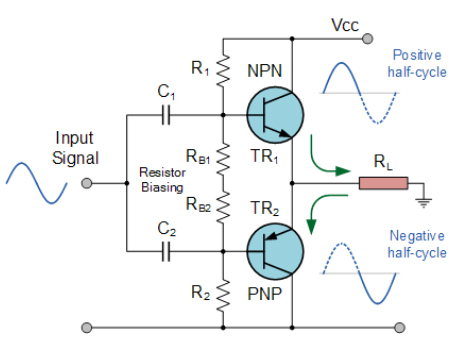
\includegraphics[scale=0.5]{IMG/AmpB.jpg}
          \caption{Amplificador de clase B}
        \end{figure}
        Esto da como resultado que cada transistor solo amplifica un semiciclo de 180 grados o en otras palabras, la mitad de la onda. Esto da como resultado que haya un pequeño lapso donde la señal queda en 0, por tanto hay una pequña deistorcion de la señal original.\\
        \begin{center}
            \textbf{Configuraciones de amplificadores clase B: Push-Pull.}
        \end{center}
            En este tipo de amplificador la corriente de carga se comparte entre los dos trancistores reduciendo el voltaje y la corriente de salida a cero mientras se comparten la onda. Como resultado se tiene que duplica la eficiencia del Amplificador clase A en hasta un 70\%\\\\
        \begin{figure}[htbp]
            \centering
            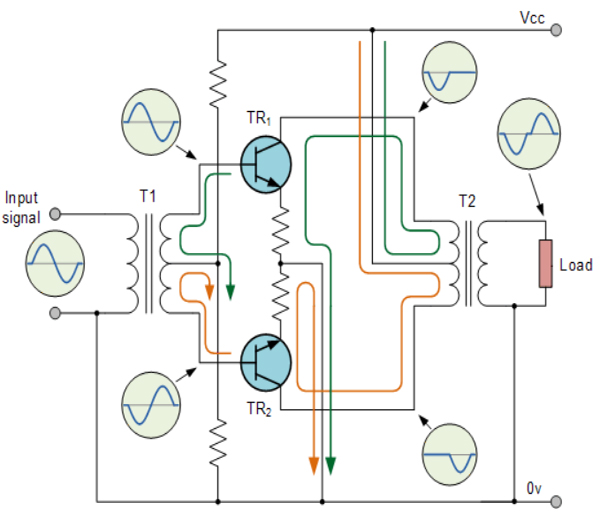
\includegraphics[scale=0.5]{IMG/AmpTPP.jpg}
            \caption{Amplificador Push-Pull o clase B estandar.}
            \label{fig:cir1}
        \end{figure}
            Este amplificador tiene la ventaja de que ninguna corriente fluye a traves de el cuando los trancistores estan en reposo por lo tanto no se disipa potencia en forma de calor.\\\\
            \begin{figure}[htbp]
                \centering
                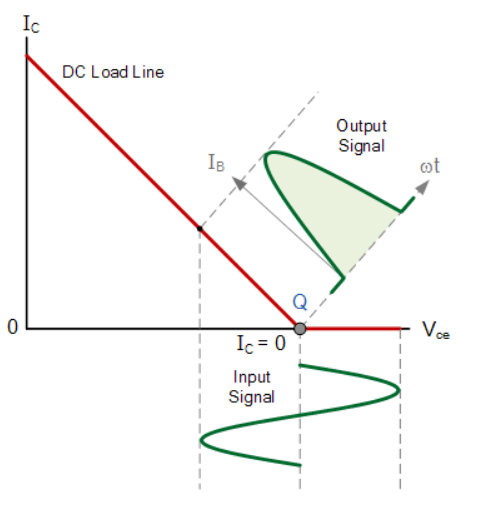
\includegraphics[scale=0.5]{IMG/CURVB}
                \caption{Curva caracteristica de la salida Clase B.}
            \end{figure} \newpage
        \begin{center}
            \textbf{Amplificador Clase AB}
        \end{center}
        El circuto de Amplificacion Clase AB es una convinacion entre el, obviamente, A y B. Una vez alcanzado el voltaje de polarizacion de los didos se conduce ligeramente incluso si no hay señal de entrda presente.\
        \begin{figure}[htbp]
            \centering
            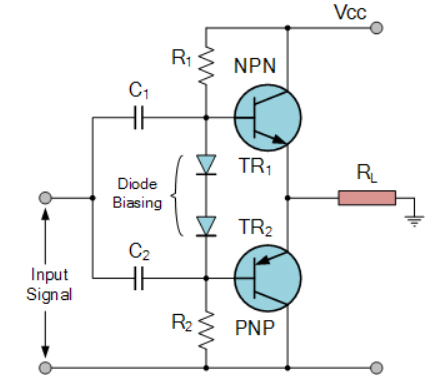
\includegraphics[scale=0.5]{IMG/AmpAB.jpg}
            \caption{Amplificador Clase AB.}
            \label{fig:cir2}
        \end{figure}
        \end{large}
\end{document}